% Options for packages loaded elsewhere
\PassOptionsToPackage{unicode}{hyperref}
\PassOptionsToPackage{hyphens}{url}
%
\documentclass[
]{article}
\usepackage{amsmath,amssymb}
\usepackage{iftex}
\ifPDFTeX
  \usepackage[T1]{fontenc}
  \usepackage[utf8]{inputenc}
  \usepackage{textcomp} % provide euro and other symbols
\else % if luatex or xetex
  \usepackage{unicode-math} % this also loads fontspec
  \defaultfontfeatures{Scale=MatchLowercase}
  \defaultfontfeatures[\rmfamily]{Ligatures=TeX,Scale=1}
\fi
\usepackage{lmodern}
\ifPDFTeX\else
  % xetex/luatex font selection
\fi
% Use upquote if available, for straight quotes in verbatim environments
\IfFileExists{upquote.sty}{\usepackage{upquote}}{}
\IfFileExists{microtype.sty}{% use microtype if available
  \usepackage[]{microtype}
  \UseMicrotypeSet[protrusion]{basicmath} % disable protrusion for tt fonts
}{}
\makeatletter
\@ifundefined{KOMAClassName}{% if non-KOMA class
  \IfFileExists{parskip.sty}{%
    \usepackage{parskip}
  }{% else
    \setlength{\parindent}{0pt}
    \setlength{\parskip}{6pt plus 2pt minus 1pt}}
}{% if KOMA class
  \KOMAoptions{parskip=half}}
\makeatother
\usepackage{xcolor}
\usepackage[margin=1in]{geometry}
\usepackage{color}
\usepackage{fancyvrb}
\newcommand{\VerbBar}{|}
\newcommand{\VERB}{\Verb[commandchars=\\\{\}]}
\DefineVerbatimEnvironment{Highlighting}{Verbatim}{commandchars=\\\{\}}
% Add ',fontsize=\small' for more characters per line
\usepackage{framed}
\definecolor{shadecolor}{RGB}{248,248,248}
\newenvironment{Shaded}{\begin{snugshade}}{\end{snugshade}}
\newcommand{\AlertTok}[1]{\textcolor[rgb]{0.94,0.16,0.16}{#1}}
\newcommand{\AnnotationTok}[1]{\textcolor[rgb]{0.56,0.35,0.01}{\textbf{\textit{#1}}}}
\newcommand{\AttributeTok}[1]{\textcolor[rgb]{0.77,0.63,0.00}{#1}}
\newcommand{\BaseNTok}[1]{\textcolor[rgb]{0.00,0.00,0.81}{#1}}
\newcommand{\BuiltInTok}[1]{#1}
\newcommand{\CharTok}[1]{\textcolor[rgb]{0.31,0.60,0.02}{#1}}
\newcommand{\CommentTok}[1]{\textcolor[rgb]{0.56,0.35,0.01}{\textit{#1}}}
\newcommand{\CommentVarTok}[1]{\textcolor[rgb]{0.56,0.35,0.01}{\textbf{\textit{#1}}}}
\newcommand{\ConstantTok}[1]{\textcolor[rgb]{0.00,0.00,0.00}{#1}}
\newcommand{\ControlFlowTok}[1]{\textcolor[rgb]{0.13,0.29,0.53}{\textbf{#1}}}
\newcommand{\DataTypeTok}[1]{\textcolor[rgb]{0.13,0.29,0.53}{#1}}
\newcommand{\DecValTok}[1]{\textcolor[rgb]{0.00,0.00,0.81}{#1}}
\newcommand{\DocumentationTok}[1]{\textcolor[rgb]{0.56,0.35,0.01}{\textbf{\textit{#1}}}}
\newcommand{\ErrorTok}[1]{\textcolor[rgb]{0.64,0.00,0.00}{\textbf{#1}}}
\newcommand{\ExtensionTok}[1]{#1}
\newcommand{\FloatTok}[1]{\textcolor[rgb]{0.00,0.00,0.81}{#1}}
\newcommand{\FunctionTok}[1]{\textcolor[rgb]{0.00,0.00,0.00}{#1}}
\newcommand{\ImportTok}[1]{#1}
\newcommand{\InformationTok}[1]{\textcolor[rgb]{0.56,0.35,0.01}{\textbf{\textit{#1}}}}
\newcommand{\KeywordTok}[1]{\textcolor[rgb]{0.13,0.29,0.53}{\textbf{#1}}}
\newcommand{\NormalTok}[1]{#1}
\newcommand{\OperatorTok}[1]{\textcolor[rgb]{0.81,0.36,0.00}{\textbf{#1}}}
\newcommand{\OtherTok}[1]{\textcolor[rgb]{0.56,0.35,0.01}{#1}}
\newcommand{\PreprocessorTok}[1]{\textcolor[rgb]{0.56,0.35,0.01}{\textit{#1}}}
\newcommand{\RegionMarkerTok}[1]{#1}
\newcommand{\SpecialCharTok}[1]{\textcolor[rgb]{0.00,0.00,0.00}{#1}}
\newcommand{\SpecialStringTok}[1]{\textcolor[rgb]{0.31,0.60,0.02}{#1}}
\newcommand{\StringTok}[1]{\textcolor[rgb]{0.31,0.60,0.02}{#1}}
\newcommand{\VariableTok}[1]{\textcolor[rgb]{0.00,0.00,0.00}{#1}}
\newcommand{\VerbatimStringTok}[1]{\textcolor[rgb]{0.31,0.60,0.02}{#1}}
\newcommand{\WarningTok}[1]{\textcolor[rgb]{0.56,0.35,0.01}{\textbf{\textit{#1}}}}
\usepackage{graphicx}
\makeatletter
\def\maxwidth{\ifdim\Gin@nat@width>\linewidth\linewidth\else\Gin@nat@width\fi}
\def\maxheight{\ifdim\Gin@nat@height>\textheight\textheight\else\Gin@nat@height\fi}
\makeatother
% Scale images if necessary, so that they will not overflow the page
% margins by default, and it is still possible to overwrite the defaults
% using explicit options in \includegraphics[width, height, ...]{}
\setkeys{Gin}{width=\maxwidth,height=\maxheight,keepaspectratio}
% Set default figure placement to htbp
\makeatletter
\def\fps@figure{htbp}
\makeatother
\setlength{\emergencystretch}{3em} % prevent overfull lines
\providecommand{\tightlist}{%
  \setlength{\itemsep}{0pt}\setlength{\parskip}{0pt}}
\setcounter{secnumdepth}{-\maxdimen} % remove section numbering
\ifLuaTeX
  \usepackage{selnolig}  % disable illegal ligatures
\fi
\IfFileExists{bookmark.sty}{\usepackage{bookmark}}{\usepackage{hyperref}}
\IfFileExists{xurl.sty}{\usepackage{xurl}}{} % add URL line breaks if available
\urlstyle{same}
\hypersetup{
  pdftitle={Artificial Intelligence Opinion Survey},
  pdfauthor={Mentor: Dr.~Nicholas Dietrich Aadarsha Gopala Reddy, Darren Lo, Ethan Love, Jose Mancilla, Santo Sumo},
  hidelinks,
  pdfcreator={LaTeX via pandoc}}

\title{Artificial Intelligence Opinion Survey}
\usepackage{etoolbox}
\makeatletter
\providecommand{\subtitle}[1]{% add subtitle to \maketitle
  \apptocmd{\@title}{\par {\large #1 \par}}{}{}
}
\makeatother
\subtitle{DATA 490 Independent Study}
\author{Mentor: Dr.~Nicholas Dietrich\\
Aadarsha Gopala Reddy, Darren Lo,\\
Ethan Love, Jose Mancilla, Santo Sumo}
\date{April 20, 2023}

\begin{document}
\maketitle

{
\setcounter{tocdepth}{2}
\tableofcontents
}
\hypertarget{load-data}{%
\section{1. Load Data}\label{load-data}}

\begin{Shaded}
\begin{Highlighting}[]
\FunctionTok{library}\NormalTok{(tidyverse)}
\end{Highlighting}
\end{Shaded}

\begin{verbatim}
## -- Attaching packages --------------------------------------- tidyverse 1.3.2 --
## v ggplot2 3.4.1     v purrr   1.0.1
## v tibble  3.1.8     v dplyr   1.1.0
## v tidyr   1.3.0     v stringr 1.5.0
## v readr   2.1.4     v forcats 1.0.0
## -- Conflicts ------------------------------------------ tidyverse_conflicts() --
## x dplyr::filter() masks stats::filter()
## x dplyr::lag()    masks stats::lag()
\end{verbatim}

\begin{Shaded}
\begin{Highlighting}[]
\FunctionTok{library}\NormalTok{(ggplot2)}

\CommentTok{\# Load data. Top row is column name.}
\NormalTok{edu }\OtherTok{\textless{}{-}} \FunctionTok{read.csv}\NormalTok{(}\StringTok{"prolific\_edu.csv"}\NormalTok{)}
\NormalTok{health }\OtherTok{\textless{}{-}} \FunctionTok{read.csv}\NormalTok{(}\StringTok{"prolific\_health.csv"}\NormalTok{)}
\NormalTok{retail }\OtherTok{\textless{}{-}} \FunctionTok{read.csv}\NormalTok{(}\StringTok{"prolific\_retail.csv"}\NormalTok{)}
\NormalTok{tech }\OtherTok{\textless{}{-}} \FunctionTok{read.csv}\NormalTok{(}\StringTok{"prolific\_tech.csv"}\NormalTok{)}
\NormalTok{qualtrics }\OtherTok{\textless{}{-}} \FunctionTok{read.csv}\NormalTok{(}\StringTok{"qualtrics\_data.csv"}\NormalTok{)}
\end{Highlighting}
\end{Shaded}

\hypertarget{data-cleaning}{%
\section{2. Data Cleaning}\label{data-cleaning}}

\begin{Shaded}
\begin{Highlighting}[]
\CommentTok{\# Combine data into one data frame after mutating Age to be one data type}
\NormalTok{edu }\OtherTok{\textless{}{-}}\NormalTok{ edu }\SpecialCharTok{\%\textgreater{}\%} \FunctionTok{mutate}\NormalTok{(}\AttributeTok{Age =} \FunctionTok{as.character}\NormalTok{(Age))}
\NormalTok{health }\OtherTok{\textless{}{-}}\NormalTok{ health }\SpecialCharTok{\%\textgreater{}\%} \FunctionTok{mutate}\NormalTok{(}\AttributeTok{Age =} \FunctionTok{as.character}\NormalTok{(Age))}
\NormalTok{retail }\OtherTok{\textless{}{-}}\NormalTok{ retail }\SpecialCharTok{\%\textgreater{}\%} \FunctionTok{mutate}\NormalTok{(}\AttributeTok{Age =} \FunctionTok{as.character}\NormalTok{(Age))}
\NormalTok{tech }\OtherTok{\textless{}{-}}\NormalTok{ tech }\SpecialCharTok{\%\textgreater{}\%} \FunctionTok{mutate}\NormalTok{(}\AttributeTok{Age =} \FunctionTok{as.character}\NormalTok{(Age))}

\NormalTok{combined }\OtherTok{\textless{}{-}} \FunctionTok{bind\_rows}\NormalTok{(edu, health, retail, tech)}
\CommentTok{\# export combined data to csv}
\CommentTok{\# write.csv(combined, "combined\_non\_qualtrics.csv")}
\end{Highlighting}
\end{Shaded}

\begin{Shaded}
\begin{Highlighting}[]
\CommentTok{\# combine qualtrics and combined data using qualtrics data\textquotesingle{}s}
\CommentTok{\#     ProlificID column and combined data\textquotesingle{}s Participant id}
\NormalTok{combined }\OtherTok{\textless{}{-}} \FunctionTok{left\_join}\NormalTok{(qualtrics, combined, }\AttributeTok{by =} \FunctionTok{c}\NormalTok{(}\StringTok{"ProlificID"} \OtherTok{=} \StringTok{"Participant.id"}\NormalTok{))}
\CommentTok{\# rename "Duration..in.seconds." column to "Duration"}
\FunctionTok{colnames}\NormalTok{(combined)[}\FunctionTok{colnames}\NormalTok{(combined) }\SpecialCharTok{==} \StringTok{"Duration..in.seconds."}\NormalTok{] }\OtherTok{\textless{}{-}} \StringTok{"Duration"}
\CommentTok{\# remove Age.x and keep only Age.y column and rename Age.y to Age}
\NormalTok{combined }\OtherTok{\textless{}{-}}\NormalTok{ combined }\SpecialCharTok{\%\textgreater{}\%}
  \FunctionTok{select}\NormalTok{(}\SpecialCharTok{{-}}\NormalTok{Age.x) }\SpecialCharTok{\%\textgreater{}\%}
  \FunctionTok{rename}\NormalTok{(}\AttributeTok{Age =}\NormalTok{ Age.y)}
\CommentTok{\# remove Status.x and Status.y columns}
\NormalTok{combined }\OtherTok{\textless{}{-}}\NormalTok{ combined }\SpecialCharTok{\%\textgreater{}\%}
  \FunctionTok{select}\NormalTok{(}\SpecialCharTok{{-}}\NormalTok{Status.x) }\SpecialCharTok{\%\textgreater{}\%}
  \FunctionTok{select}\NormalTok{(}\SpecialCharTok{{-}}\NormalTok{Status.y)}
\CommentTok{\# remove Finished, Progress, UserLanguage, DistributionChannel,}
\CommentTok{\# Nationality, and Consent columns}
\NormalTok{combined }\OtherTok{\textless{}{-}}\NormalTok{ combined }\SpecialCharTok{\%\textgreater{}\%}
  \FunctionTok{select}\NormalTok{(}\SpecialCharTok{{-}}\NormalTok{Finished) }\SpecialCharTok{\%\textgreater{}\%}
  \FunctionTok{select}\NormalTok{(}\SpecialCharTok{{-}}\NormalTok{Progress) }\SpecialCharTok{\%\textgreater{}\%}
  \FunctionTok{select}\NormalTok{(}\SpecialCharTok{{-}}\NormalTok{UserLanguage) }\SpecialCharTok{\%\textgreater{}\%}
  \FunctionTok{select}\NormalTok{(}\SpecialCharTok{{-}}\NormalTok{DistributionChannel) }\SpecialCharTok{\%\textgreater{}\%}
  \FunctionTok{select}\NormalTok{(}\SpecialCharTok{{-}}\NormalTok{Nationality) }\SpecialCharTok{\%\textgreater{}\%}
  \FunctionTok{select}\NormalTok{(}\SpecialCharTok{{-}}\NormalTok{Consent)}


\CommentTok{\# remove rows where Submission.id is NA}
\NormalTok{combined }\OtherTok{\textless{}{-}}\NormalTok{ combined }\SpecialCharTok{\%\textgreater{}\%} \FunctionTok{filter}\NormalTok{(}\SpecialCharTok{!}\FunctionTok{is.na}\NormalTok{(Submission.id))}
\CommentTok{\# Keep only rows which say "United States" in "Country.of.residence" column}
\NormalTok{combined }\OtherTok{\textless{}{-}}\NormalTok{ combined }\SpecialCharTok{\%\textgreater{}\%} \FunctionTok{filter}\NormalTok{(combined}\SpecialCharTok{$}\NormalTok{Country.of.residence }\SpecialCharTok{==} \StringTok{"United States"}\NormalTok{)}
\CommentTok{\# Replace all cells that say "Information Technology" and "Science, Technology, Engineering \& Mathematics" to "STEM/IT" in Employment.sector column}
\NormalTok{combined}\SpecialCharTok{$}\NormalTok{Employment.sector[combined}\SpecialCharTok{$}\NormalTok{Employment.sector }\SpecialCharTok{==} \StringTok{"Information Technology"}\NormalTok{] }\OtherTok{\textless{}{-}} \StringTok{"STEM/IT"}
\NormalTok{combined}\SpecialCharTok{$}\NormalTok{Employment.sector[combined}\SpecialCharTok{$}\NormalTok{Employment.sector }\SpecialCharTok{==} \StringTok{"Science, Technology, Engineering \& Mathematics"}\NormalTok{] }\OtherTok{\textless{}{-}} \StringTok{"STEM/IT"}

\CommentTok{\# change all cells in column EnhanceHurt that say "AI will neither enhance nor detract from my work" to "neither", "AI will enhance my work" to "enhance", and "AI will detract from my work" to "detract"}
\NormalTok{combined}\SpecialCharTok{$}\NormalTok{EnhanceHurt[combined}\SpecialCharTok{$}\NormalTok{EnhanceHurt }\SpecialCharTok{==} \StringTok{"AI will neither enhance nor detract from my work"}\NormalTok{] }\OtherTok{\textless{}{-}} \StringTok{"neither"}
\NormalTok{combined}\SpecialCharTok{$}\NormalTok{EnhanceHurt[combined}\SpecialCharTok{$}\NormalTok{EnhanceHurt }\SpecialCharTok{==} \StringTok{"AI will enhance my work"}\NormalTok{] }\OtherTok{\textless{}{-}} \StringTok{"enhance"}
\NormalTok{combined}\SpecialCharTok{$}\NormalTok{EnhanceHurt[combined}\SpecialCharTok{$}\NormalTok{EnhanceHurt }\SpecialCharTok{==} \StringTok{"AI will detract from my work"}\NormalTok{] }\OtherTok{\textless{}{-}} \StringTok{"detract"}

\CommentTok{\# export data to csv}
\CommentTok{\# write.csv(combined, "combined\_qualtrics.csv")}
\end{Highlighting}
\end{Shaded}

\begin{Shaded}
\begin{Highlighting}[]
\CommentTok{\# Keep only rows which say "Compose an email" in "Attention" column}
\NormalTok{combined }\OtherTok{\textless{}{-}}\NormalTok{ combined }\SpecialCharTok{\%\textgreater{}\%} \FunctionTok{filter}\NormalTok{(combined}\SpecialCharTok{$}\NormalTok{Attention }\SpecialCharTok{==} \StringTok{"Compose an email"}\NormalTok{)}
\CommentTok{\# remove Attention column}
\NormalTok{combined }\OtherTok{\textless{}{-}}\NormalTok{ combined }\SpecialCharTok{\%\textgreater{}\%} \FunctionTok{select}\NormalTok{(}\SpecialCharTok{{-}}\NormalTok{Attention)}
\CommentTok{\# export data to csv}
\CommentTok{\# write.csv(combined, "combined\_qualtrics\_attentive.csv")}
\end{Highlighting}
\end{Shaded}

\hypertarget{data-exploration}{%
\section{3. Data Exploration}\label{data-exploration}}

The columns in the dataset are:

\begin{itemize}
\item
  \emph{StartDate} - Date and time survey was started
\item
  \emph{EndDate} - Date and time survey was completed
\item
  \emph{IPAddress} - IP address of participant
\item
  \emph{Duration} - Duration of survey in seconds
\item
  \emph{RecordedDate} - Date and time survey was recorded
\item
  \emph{ResponseId} - Response ID
\item
  \emph{LocationLatitude} - Participant's location latitude
\item
  \emph{LocationLongitude} - Participant's location longitude
\item
  \emph{ProlificID} - Identification of the response on Prolific
\item
  \emph{Gender} - Gender of the participant
\item
  \emph{Education} - Education level of the participant
\item
  \emph{Salary} - Salary of the participant
\item
  \emph{AIKnowledge} - Knowledge of AI of the participant
\item
  \emph{UsedAI} - Whether the participant has used AI
\item
  \emph{TimeEnergy} - How much time and energy AI has saved the
  participant
\item
  \emph{SimilarTasks} - How much of the participant's tasks they think
  AI can do
\item
  \emph{EnhanceHurt} - Whether the participant thinks AI can enhance or
  hurt their work efficiency.
\item
  \emph{Comments} - Comments from the participant
\item
  \emph{Submission.id} - Submission ID
\item
  \emph{Started.at} - Date and time survey was started
\item
  \emph{Completed.at} - Date and time survey was completed
\item
  \emph{Reviewed.at} - Date and time survey was reviewed
\item
  \emph{Archived.at} - Date and time survey was archived
\item
  \emph{Time.taken} - Duration of survey in seconds
\item
  \emph{Completion.code} - Completion code
\item
  \emph{Total.approvals} - Total number of approvals
\item
  \emph{Employment.sector} - Employment sector
\item
  \emph{Age} - Age of the participant
\item
  \emph{Sex} - Sex of the participant
\item
  \emph{Ethnicity.simplified} - Ethnicity of the participant
\item
  \emph{Country.of.birth} - Country of birth of the participant
\item
  \emph{Country.of.residence} - Country of residence of the participant
\item
  \emph{Language} - Language of the participant
\item
  \emph{Student.status} - Whether the participant is a student
\item
  \emph{Employment.status} - Whether the participant is employed
\end{itemize}

\hypertarget{data-analysis}{%
\section{4. Data Analysis}\label{data-analysis}}

\hypertarget{enhancehurt-vs.-industry-proportions}{%
\subsection{4.1. EnhanceHurt vs.~Industry
(proportions)}\label{enhancehurt-vs.-industry-proportions}}

\begin{Shaded}
\begin{Highlighting}[]
\CommentTok{\# Create a new data frame with only the columns we need}
\NormalTok{enhancehurt\_vs\_industry }\OtherTok{\textless{}{-}}\NormalTok{ combined }\SpecialCharTok{\%\textgreater{}\%} \FunctionTok{select}\NormalTok{(EnhanceHurt, Employment.sector)}

\CommentTok{\# Remove rows where Employment.sector is NA}
\NormalTok{enhancehurt\_vs\_industry }\OtherTok{\textless{}{-}}\NormalTok{ enhancehurt\_vs\_industry }\SpecialCharTok{\%\textgreater{}\%} \FunctionTok{filter}\NormalTok{(}\SpecialCharTok{!}\FunctionTok{is.na}\NormalTok{(Employment.sector))}
\CommentTok{\# Remove rows where EnhanceHurt is NA}
\NormalTok{enhancehurt\_vs\_industry }\OtherTok{\textless{}{-}}\NormalTok{ enhancehurt\_vs\_industry }\SpecialCharTok{\%\textgreater{}\%} \FunctionTok{filter}\NormalTok{(}\SpecialCharTok{!}\FunctionTok{is.na}\NormalTok{(EnhanceHurt))}

\CommentTok{\# For each industry, calculate the proportion of respondents who think AI can enhance their work efficiency}
\NormalTok{enhancehurt\_vs\_industry }\OtherTok{\textless{}{-}}\NormalTok{ enhancehurt\_vs\_industry }\SpecialCharTok{\%\textgreater{}\%}
  \FunctionTok{group\_by}\NormalTok{(Employment.sector, EnhanceHurt) }\SpecialCharTok{\%\textgreater{}\%}
  \FunctionTok{summarize}\NormalTok{(}\AttributeTok{count =} \FunctionTok{n}\NormalTok{()) }\SpecialCharTok{\%\textgreater{}\%}
  \FunctionTok{mutate}\NormalTok{(}\AttributeTok{prop =}\NormalTok{ count }\SpecialCharTok{/} \FunctionTok{sum}\NormalTok{(count))}
\end{Highlighting}
\end{Shaded}

\begin{verbatim}
## `summarise()` has grouped output by 'Employment.sector'. You can override using
## the `.groups` argument.
\end{verbatim}

\begin{Shaded}
\begin{Highlighting}[]
\CommentTok{\# Visualize using different histogram for each industry.}
\CommentTok{\# Show the number of respondents inside each bar.}
\CommentTok{\# make legend bottom. Wrap x axis labels without changing plot size.}
\NormalTok{enhancehurt\_vs\_industry\_plot }\OtherTok{\textless{}{-}} \FunctionTok{ggplot}\NormalTok{(enhancehurt\_vs\_industry, }\FunctionTok{aes}\NormalTok{(}
  \AttributeTok{x =}\NormalTok{ Employment.sector,}
  \AttributeTok{y =}\NormalTok{ prop, }\AttributeTok{fill =}\NormalTok{ EnhanceHurt}
\NormalTok{)) }\SpecialCharTok{+}
  \FunctionTok{geom\_bar}\NormalTok{(}\AttributeTok{stat =} \StringTok{"identity"}\NormalTok{, }\AttributeTok{position =} \StringTok{"dodge"}\NormalTok{) }\SpecialCharTok{+}
  \FunctionTok{geom\_text}\NormalTok{(}\FunctionTok{aes}\NormalTok{(}\AttributeTok{label =}\NormalTok{ count),}
    \AttributeTok{position =} \FunctionTok{position\_dodge}\NormalTok{(}\AttributeTok{width =} \DecValTok{1}\NormalTok{),}
    \AttributeTok{vjust =} \FloatTok{1.5}
\NormalTok{  ) }\SpecialCharTok{+}
  \FunctionTok{labs}\NormalTok{(}
    \AttributeTok{x =} \StringTok{"Industry"}\NormalTok{, }\AttributeTok{y =} \StringTok{"Proportion of Respondents"}\NormalTok{,}
    \AttributeTok{fill =} \StringTok{"Enhance or Hurt"}
\NormalTok{  ) }\SpecialCharTok{+}
  \FunctionTok{ggtitle}\NormalTok{(}\StringTok{"Proportion of Respondents Who Think AI Can}\SpecialCharTok{\textbackslash{}n}
\StringTok{  Enhance Their Work Efficiency by Industry"}\NormalTok{) }\SpecialCharTok{+}
  \FunctionTok{theme}\NormalTok{(}
    \AttributeTok{plot.title =} \FunctionTok{element\_text}\NormalTok{(}\AttributeTok{hjust =} \FloatTok{0.5}\NormalTok{),}
    \AttributeTok{legend.position =} \StringTok{"bottom"}
\NormalTok{  )}

\NormalTok{enhancehurt\_vs\_industry\_plot}
\end{Highlighting}
\end{Shaded}

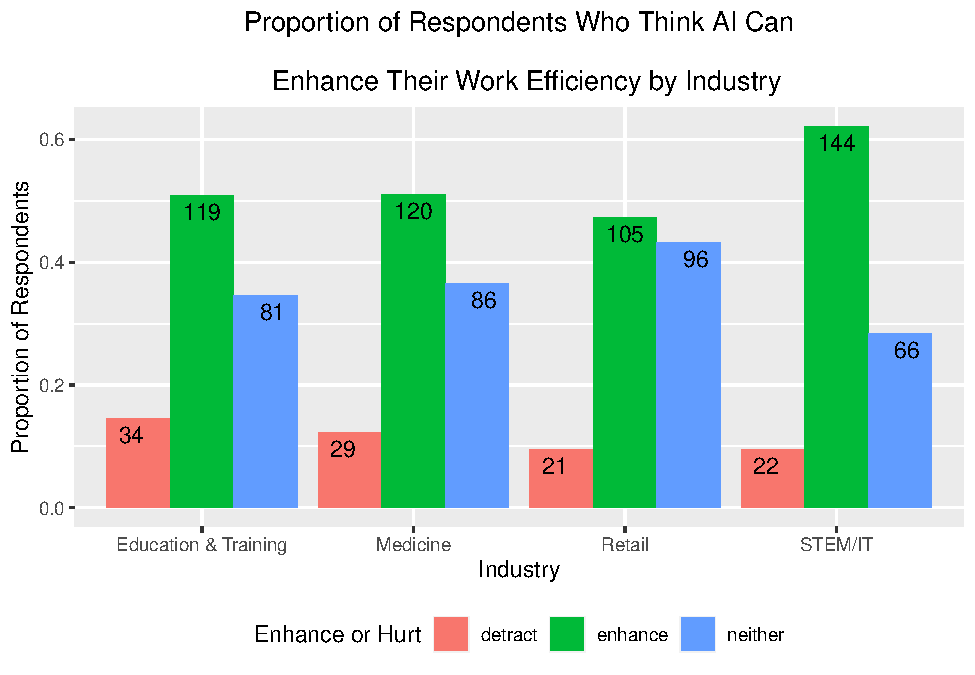
\includegraphics{analysis_files/figure-latex/enhancehurt-vs-industry-1.pdf}

\hypertarget{enhancehurt-vs.-education-proportions}{%
\subsection{4.2. EnhanceHurt vs.~Education
(proportions)}\label{enhancehurt-vs.-education-proportions}}

\begin{Shaded}
\begin{Highlighting}[]
\CommentTok{\# Create a new data frame with only the columns we need}
\NormalTok{enhancehurt\_vs\_education }\OtherTok{\textless{}{-}}\NormalTok{ combined }\SpecialCharTok{\%\textgreater{}\%} \FunctionTok{select}\NormalTok{(EnhanceHurt, Education)}

\CommentTok{\# Remove rows where Education is NA}
\NormalTok{enhancehurt\_vs\_education }\OtherTok{\textless{}{-}}\NormalTok{ enhancehurt\_vs\_education }\SpecialCharTok{\%\textgreater{}\%} \FunctionTok{filter}\NormalTok{(}\SpecialCharTok{!}\FunctionTok{is.na}\NormalTok{(Education))}
\CommentTok{\# Remove rows where EnhanceHurt is NA}
\NormalTok{enhancehurt\_vs\_education }\OtherTok{\textless{}{-}}\NormalTok{ enhancehurt\_vs\_education }\SpecialCharTok{\%\textgreater{}\%} \FunctionTok{filter}\NormalTok{(}\SpecialCharTok{!}\FunctionTok{is.na}\NormalTok{(EnhanceHurt))}

\CommentTok{\# For each education level, calculate the proportion of respondents who think AI can enhance their work efficiency}
\NormalTok{enhancehurt\_vs\_education }\OtherTok{\textless{}{-}}\NormalTok{ enhancehurt\_vs\_education }\SpecialCharTok{\%\textgreater{}\%}
  \FunctionTok{group\_by}\NormalTok{(Education, EnhanceHurt) }\SpecialCharTok{\%\textgreater{}\%}
  \FunctionTok{summarize}\NormalTok{(}\AttributeTok{count =} \FunctionTok{n}\NormalTok{()) }\SpecialCharTok{\%\textgreater{}\%}
  \FunctionTok{mutate}\NormalTok{(}\AttributeTok{prop =}\NormalTok{ count }\SpecialCharTok{/} \FunctionTok{sum}\NormalTok{(count))}
\end{Highlighting}
\end{Shaded}

\begin{verbatim}
## `summarise()` has grouped output by 'Education'. You can override using the
## `.groups` argument.
\end{verbatim}

\begin{Shaded}
\begin{Highlighting}[]
\CommentTok{\# Visualize using different histogram for each education level.}
\CommentTok{\# Show the number of respondents on each bar.}
\NormalTok{enhancehurt\_vs\_education\_plot }\OtherTok{\textless{}{-}} \FunctionTok{ggplot}\NormalTok{(enhancehurt\_vs\_education, }\FunctionTok{aes}\NormalTok{(}
  \AttributeTok{x =}\NormalTok{ Education, }\AttributeTok{y =}\NormalTok{ prop,}
  \AttributeTok{fill =}\NormalTok{ EnhanceHurt}
\NormalTok{)) }\SpecialCharTok{+}
  \FunctionTok{geom\_bar}\NormalTok{(}\AttributeTok{stat =} \StringTok{"identity"}\NormalTok{, }\AttributeTok{position =} \StringTok{"dodge"}\NormalTok{) }\SpecialCharTok{+}
  \FunctionTok{geom\_text}\NormalTok{(}\FunctionTok{aes}\NormalTok{(}\AttributeTok{label =}\NormalTok{ count),}
    \AttributeTok{position =} \FunctionTok{position\_dodge}\NormalTok{(}\AttributeTok{width =} \DecValTok{1}\NormalTok{),}
    \AttributeTok{vjust =} \FloatTok{1.5}
\NormalTok{  ) }\SpecialCharTok{+}
  \FunctionTok{labs}\NormalTok{(}
    \AttributeTok{x =} \StringTok{"Education Level"}\NormalTok{, }\AttributeTok{y =} \StringTok{"Proportion of Respondents"}\NormalTok{,}
    \AttributeTok{fill =} \StringTok{"Enhance or Hurt"}
\NormalTok{  ) }\SpecialCharTok{+}
  \FunctionTok{ggtitle}\NormalTok{(}\StringTok{"Proportion of Respondents Who Think AI Can}\SpecialCharTok{\textbackslash{}n}
\StringTok{  Enhance Their Work Efficiency by Education Level"}\NormalTok{) }\SpecialCharTok{+}
  \FunctionTok{theme}\NormalTok{(}\AttributeTok{plot.title =} \FunctionTok{element\_text}\NormalTok{(}\AttributeTok{hjust =} \FloatTok{0.5}\NormalTok{)) }\SpecialCharTok{+}
  \FunctionTok{theme}\NormalTok{(}\AttributeTok{legend.position =} \StringTok{"top"}\NormalTok{)}

\NormalTok{enhancehurt\_vs\_education\_plot}
\end{Highlighting}
\end{Shaded}

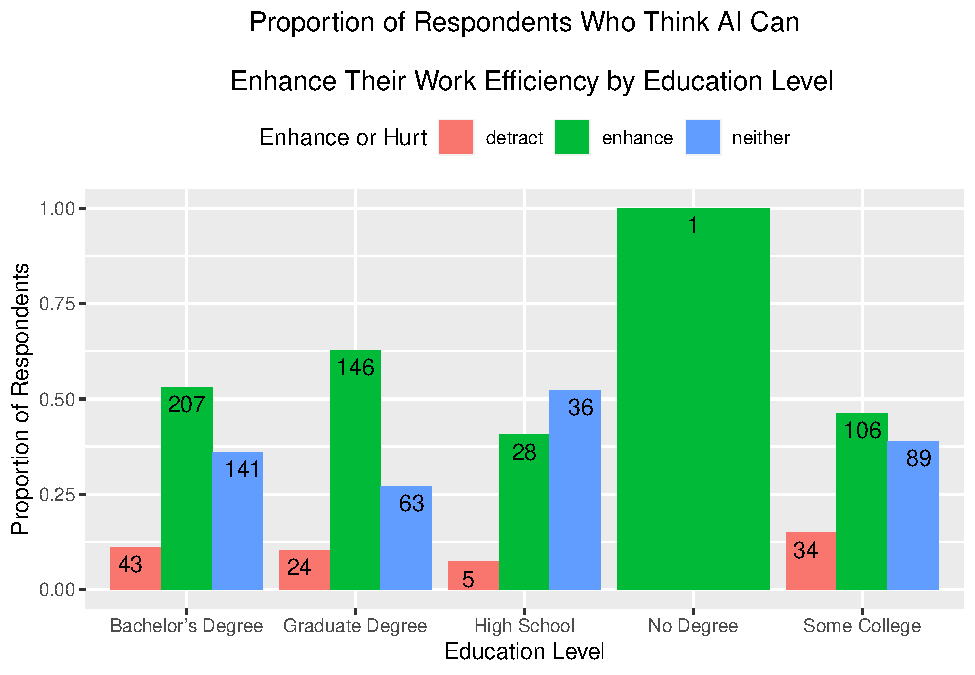
\includegraphics{analysis_files/figure-latex/enhancehurt-vs-education-1.pdf}

\hypertarget{enhancehurt-vs.-age-proportions}{%
\subsection{4.3 EnhanceHurt vs.~Age
(proportions)}\label{enhancehurt-vs.-age-proportions}}

\begin{Shaded}
\begin{Highlighting}[]
\CommentTok{\# Create a new data frame with only the columns we need}
\NormalTok{enhancehurt\_vs\_age }\OtherTok{\textless{}{-}}\NormalTok{ combined }\SpecialCharTok{\%\textgreater{}\%} \FunctionTok{select}\NormalTok{(EnhanceHurt, Age)}
\CommentTok{\# Remove the Ages which say "DATA\_EXPIRED" and "923"}
\NormalTok{enhancehurt\_vs\_age }\OtherTok{\textless{}{-}}\NormalTok{ enhancehurt\_vs\_age }\SpecialCharTok{\%\textgreater{}\%} \FunctionTok{filter}\NormalTok{(enhancehurt\_vs\_age}\SpecialCharTok{$}\NormalTok{Age }\SpecialCharTok{!=} \StringTok{"DATA\_EXPIRED"}\NormalTok{)}
\NormalTok{enhancehurt\_vs\_age }\OtherTok{\textless{}{-}}\NormalTok{ enhancehurt\_vs\_age }\SpecialCharTok{\%\textgreater{}\%} \FunctionTok{filter}\NormalTok{(enhancehurt\_vs\_age}\SpecialCharTok{$}\NormalTok{Age }\SpecialCharTok{!=} \StringTok{"923"}\NormalTok{)}

\CommentTok{\# Remove rows where Age is NA}
\NormalTok{enhancehurt\_vs\_age }\OtherTok{\textless{}{-}}\NormalTok{ enhancehurt\_vs\_age }\SpecialCharTok{\%\textgreater{}\%} \FunctionTok{filter}\NormalTok{(}\SpecialCharTok{!}\FunctionTok{is.na}\NormalTok{(Age))}
\CommentTok{\# Remove rows where EnhanceHurt is NA}
\NormalTok{enhancehurt\_vs\_age }\OtherTok{\textless{}{-}}\NormalTok{ enhancehurt\_vs\_age }\SpecialCharTok{\%\textgreater{}\%} \FunctionTok{filter}\NormalTok{(}\SpecialCharTok{!}\FunctionTok{is.na}\NormalTok{(EnhanceHurt))}

\CommentTok{\# Convert Age to numeric}
\NormalTok{enhancehurt\_vs\_age}\SpecialCharTok{$}\NormalTok{Age }\OtherTok{\textless{}{-}} \FunctionTok{as.numeric}\NormalTok{(}\FunctionTok{as.character}\NormalTok{(enhancehurt\_vs\_age}\SpecialCharTok{$}\NormalTok{Age))}
\CommentTok{\# group ages by 5 years}
\NormalTok{enhancehurt\_vs\_age}\SpecialCharTok{$}\NormalTok{Age }\OtherTok{\textless{}{-}} \FunctionTok{cut}\NormalTok{(enhancehurt\_vs\_age}\SpecialCharTok{$}\NormalTok{Age, }\AttributeTok{breaks =} \FunctionTok{seq}\NormalTok{(}\DecValTok{18}\NormalTok{, }\DecValTok{80}\NormalTok{, }\AttributeTok{by =} \DecValTok{10}\NormalTok{))}
\CommentTok{\# remove NA}
\NormalTok{enhancehurt\_vs\_age }\OtherTok{\textless{}{-}}\NormalTok{ enhancehurt\_vs\_age }\SpecialCharTok{\%\textgreater{}\%} \FunctionTok{filter}\NormalTok{(}\SpecialCharTok{!}\FunctionTok{is.na}\NormalTok{(Age))}

\CommentTok{\# create a new dataframe with the proportion of respondents who think AI can enhance their work efficiency for each age group}
\NormalTok{enhancehurt\_vs\_age }\OtherTok{\textless{}{-}}\NormalTok{ enhancehurt\_vs\_age }\SpecialCharTok{\%\textgreater{}\%}
  \FunctionTok{group\_by}\NormalTok{(Age, EnhanceHurt) }\SpecialCharTok{\%\textgreater{}\%}
  \FunctionTok{summarize}\NormalTok{(}\AttributeTok{count =} \FunctionTok{n}\NormalTok{()) }\SpecialCharTok{\%\textgreater{}\%}
  \FunctionTok{mutate}\NormalTok{(}\AttributeTok{prop =}\NormalTok{ count }\SpecialCharTok{/} \FunctionTok{sum}\NormalTok{(count))}
\end{Highlighting}
\end{Shaded}

\begin{verbatim}
## `summarise()` has grouped output by 'Age'. You can override using the `.groups`
## argument.
\end{verbatim}

\begin{Shaded}
\begin{Highlighting}[]
\CommentTok{\# Visualize using different histogram for each age group.}
\CommentTok{\# Show the number of respondents on each bar.}
\NormalTok{enhancehurt\_vs\_age\_plot }\OtherTok{\textless{}{-}} \FunctionTok{ggplot}\NormalTok{(enhancehurt\_vs\_age, }\FunctionTok{aes}\NormalTok{(}
  \AttributeTok{x =}\NormalTok{ Age, }\AttributeTok{y =}\NormalTok{ prop,}
  \AttributeTok{fill =}\NormalTok{ EnhanceHurt}
\NormalTok{)) }\SpecialCharTok{+}
  \FunctionTok{geom\_bar}\NormalTok{(}\AttributeTok{stat =} \StringTok{"identity"}\NormalTok{, }\AttributeTok{position =} \StringTok{"dodge"}\NormalTok{) }\SpecialCharTok{+}
  \FunctionTok{geom\_text}\NormalTok{(}\FunctionTok{aes}\NormalTok{(}\AttributeTok{label =}\NormalTok{ count),}
    \AttributeTok{position =} \FunctionTok{position\_dodge}\NormalTok{(}\AttributeTok{width =} \DecValTok{1}\NormalTok{),}
    \AttributeTok{vjust =} \FloatTok{1.5}
\NormalTok{  ) }\SpecialCharTok{+}
  \FunctionTok{labs}\NormalTok{(}
    \AttributeTok{x =} \StringTok{"Age Group"}\NormalTok{, }\AttributeTok{y =} \StringTok{"Proportion of Respondents"}\NormalTok{,}
    \AttributeTok{fill =} \StringTok{"Enhance or Hurt"}
\NormalTok{  ) }\SpecialCharTok{+}
  \FunctionTok{ggtitle}\NormalTok{(}\StringTok{"Proportion of Respondents Who Think AI Can}\SpecialCharTok{\textbackslash{}n}
\StringTok{  Enhance Their Work Efficiency by Age Group"}\NormalTok{) }\SpecialCharTok{+}
  \FunctionTok{theme}\NormalTok{(}\AttributeTok{plot.title =} \FunctionTok{element\_text}\NormalTok{(}\AttributeTok{hjust =} \FloatTok{0.5}\NormalTok{)) }\SpecialCharTok{+}
  \FunctionTok{theme}\NormalTok{(}\AttributeTok{legend.position =} \StringTok{"top"}\NormalTok{)}

\NormalTok{enhancehurt\_vs\_age\_plot}
\end{Highlighting}
\end{Shaded}

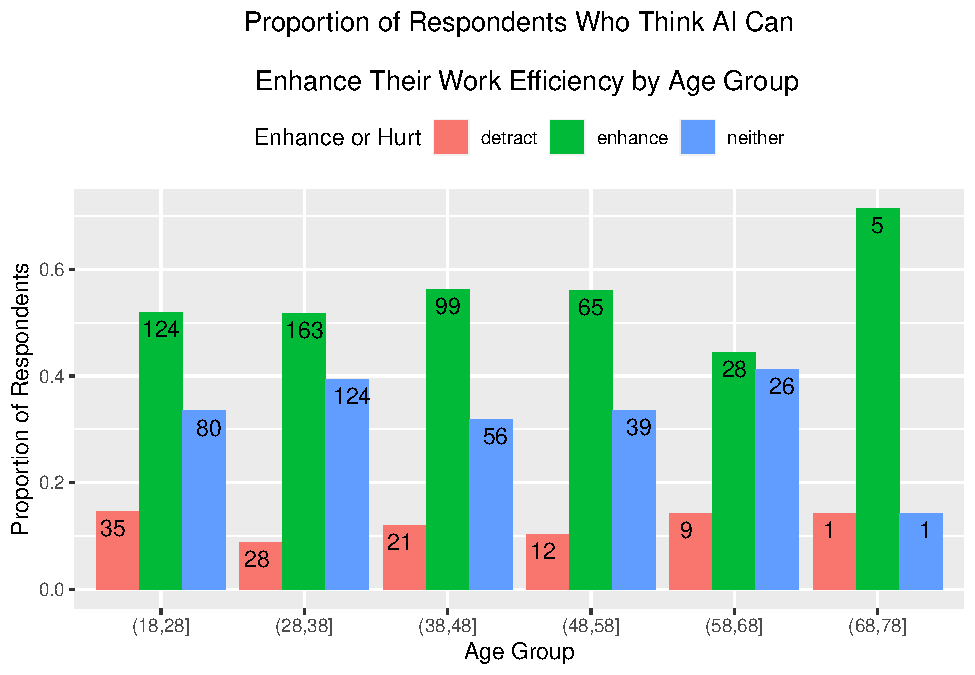
\includegraphics{analysis_files/figure-latex/enhancehurt-vs-age-1.pdf}

\end{document}
